\chapter{Поглощение света многослойной наночастицей} \label{chapt4}

\section{Введение}

Экстинкция электромагнитной волны, падающей на наночастицу,
определяется суммой рассеяния и поглощения этой же волны. Некоторые
аспекты управления рассеянием с помощью многослойных покрытий были
рассмотрены в предыдущей главе.  В настоящей главе будет рассмотрен
вопрос о фундаментальных ограничениях на эффективность поглощения
электромагнитного излучения уединённой наночастицей.

Ранее уже предпринимались попытки рассмотрения этого вопроса. В своей
работе~\cite{Tribelsky-2011} М.И. Трибельский показал, что существует
верхний предел, ограничивающий возможности поглощения для одного
мультиполя (моды). Коэффициенты Ми для поглощения электрическими
$\tilde{a}_n= {\rmfamily Re}\{a_n\} - |a_n|^2 $ и магнитными
$\tilde{b}_n= {\rmfamily Re}\{b_n\} - |b_n|^2 $ модами не могут
превысить значения $1/4$. Здесь $n=1$ соответствует случаю диполя,
$n=2$ квадрупольной моде, и так далее для больших значений $n$,
коэффициенты $a_n$ и $b_n$ имеют тот же смысл, что и в 
выражениях~\ref{eq:vector-harm1} и~\ref{eq:vector-harm2}.

Аналогичным образом, применяя только аналитические методы, Григорьев и
др.~\cite{Grigoriev-2015} рассмотрели эффект идеального поглощения на
примере двухслойной частицы, а именно случай диэлектрической сферы,
покрытой слоем золота или серебра. В дипольном приближении они
получили выражение для эффективного значения диэлектрической
проницаемости, обеспечивающего максимально достижимое поглощение в
сфере заданного размера.  В рамках теории эффективной среды
Максвелла-Гарнета ими было получено выражение для объёмной доли
диэлектрика, при которой возникает эффект идеального поглощения в
рассматриваемых двухслойных частицах.  Расчёт по этим выражениям
хорошо совпадает с расчётом по выражениям из работы
М.И. Трибельского~\cite{Tribelsky-2011} для случая $n=1$. Однако
указанный подход обладает рядом недостатков, среди которых можно
отметить ограниченную применимость (вследствие использования
дипольного приближения можно рассматривать только относительно
маленькие частицы) и то, что для большинства значений параметра
размера объёмная доля выражается комплексным числом.  Последний факт
делает эту теорию малопригодной для экспериментальной верификации.

Достоинством теории Ми является используемое разложение поля по
сферическим векторным гармоникам, что позволяет разделить вклад в
общее поле от электрической и магнитной дипольной моды, а также вклад
от квадруполей и мультиполей более высокого порядка. Таким образом,
становится возможен покомпонентный анализ спектрального отклика
многослойной сферы в зависимости от её дизайна. Например, в ряде
случаев удаётся совместить в спектре рассеяния положение нескольких
резонансов (таких как электрических дипольного и квадрупольного). Это
создаёт эффект суперрассеяния~\cite{Fan-2010,Fan-2011}, когда
многослойная частица специального дизайна рассеивает сильнее, чем
однородная частица того же размера из произвольного изотропного
материала.

В данной главе рассматривается аналогичный эффект суперпоглощения,
когда из-за совмещения нескольких резонансов сечение поглощения
сферической наночастицы превышает фундаментальный предел поглощения
мультиполя максимального порядка, возбуждённого в этой же частице.  В
этом случае, аналогично эффекту суперрассеяния, сечение поглощения
оказывается больше, чем у однородной частицы того же размера из
произвольного изотропного материала. Дело в том, что в случае
однородной сферы нет возможности совместить на одной частоте,
например, несколько электрических мод. Для заданного размера сферы из
одного материала различие в пространственной структуре низших мод
приводит к тому, что они оказываются существенно различны по
частоте. Моды высокого порядка (например моды шепчущей галлереи) могут
оказаться разнесены по частотам значительно меньше, чем ширина их
полосы в спектре, однако такие частицы оказываются гораздо больше,
перестают быть наноразмерными и не рассматриваются в настоящей
работе. Аналогичным образом оказывается невозможным совмещение на
одной частоте нескольких магнитных мод.

Последнее возможное сочетание мод для случая однородной сферы, это
совмещение электрического и магнитного резонанса. Однако для
материалов, чаще всего используемых при изготовлении наночастиц,
положение низших электрических и магнитных мод как правило не
совпадает по частоте.  Впрочем, даже если и получится подобрать
сочетание материала, размера наночастицы и используемой длины волны
(из-за наличия дисперсии в материалах приходится задавать все
парамеметры модели с размерностью длины) так, что электическая и
магнитная моды совпадут по частоте, то возможности совместить с ними
ещё одну моду не появится.  Чтобы это изменить, в систему необходимо
ввести дополнительные степени свободы, например, один или несколько
дополнительных слоёв. Такая система и является объектом рассмотрения в
настоящей главе.

\section{Результаты оптимизации}

Для изучения поглощения электромагнитной плоской волны многослойными
наночастицами использовался тот же подход, который был применён в
предыдущей главе, посвящённой изучению рассеивающих свойств.  А
именно, с помощью стохастической оптимизации были получены дизайны
наночастиц, обеспечивающие наилучшие рабочие характеристики; расчёт
эффективности поглощения при оптимизации выполнялся с помощью теории
Ми. Такой подход оказался достаточно универсальным. Он может быть
применён для широкого класса материалов, внешнего размера,
произвольного (в пределах нескольких десятков) числа слоёв
наночастицы. Однако при проведении численной оптимизации всегда
существует ограничение по доступной вычислительной мощности, что
приводят к необходимости выбора диапазона входных параметров
рассматриваемой модели. На начальном этапе были опробованы несколько
разных комбинаций используемых материалов и длин волн, был выбран
наиболее перспективный с точки зрения возможных результатов вариант. В
рамках настоящей главы было принято решение ограничиться исследованием
поглощения света только трёхслойными частицы из заранее выбранных
материалов ($Si/Ag/Si$).  Использовались экспериментально
измеренные материальные параметры~\cite{palik-1997}. Большая часть
результатов была получена для длины волны $\lambda=500$~нм,
$\varepsilon_{\rmfamily Si} = 18.5 + i 0.63$,
$\varepsilon_{\rmfamily Ag} = -8.5 + i 0.76$, а в качестве параметров
оптимизации использовать толщины составных слоёв.

Целью исследования были структуры с максимальной эффективностью
поглощения $Q_{\rmfamily abs} = C_{\rmfamily abs}/\pi R^2$ для
заданной длины волны, где $C_{\rmfamily abs}$ это сечение поглощения,
а $R$ это внешний радиус наночастицы.  Результат оптимизации для
различных значений $R$ представлен на рисунках~\ref{img:q-abs}(а--в).
В данном случае, аналогично рисунку~\ref{img:min-max-min}(б), при
работе стохастического оптимизатора удалось получить очень хороший
уровень воспроизводимости получаемых результатов. В итоге, набор
дискретных значений полученных при оптимизации, сливается с сплошные
линии, изображённые на ристунке рисунке~\ref{img:q-abs}(а). На этом
рисунке дополнительными пунктирными линиями отмечены максимально
достижимые эффективности поглощения для дипольного ($n=1$) и
квадрупольного ($n=2$) резонансов, которые определяются
зависимостью~\cite{Tribelsky-2011}
\[Q^{(n)}_{\rmfamily abs\ max}=\frac{2n+1}{2q^2}\] через параметр
размера $q=2\pi R/\lambda$.  В рассматриваемой системе максимальный
порядок резонансного возбуждения мультиполей ограничен квадруполем
($n=2$). По сравнению с ним дизайны с внешним радиусом $R>60$~нм
демонстрируют большую эффективность поглощения, то есть выполняется условие
для режима суперпоглощения.

\begin{figure}[t]
  \begin{minipage}[ht]{0.495\linewidth}
    \centering{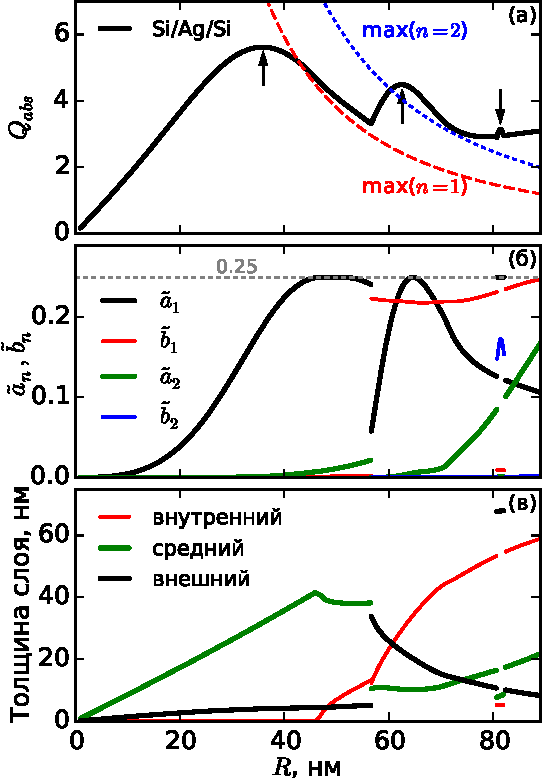
\includegraphics[height=1.35\linewidth]{2015-04-01-Qabs-SiAgSi-overview}}
  \end{minipage}
  \hfill
  \begin{minipage}[ht]{0.495\linewidth}
    \centering{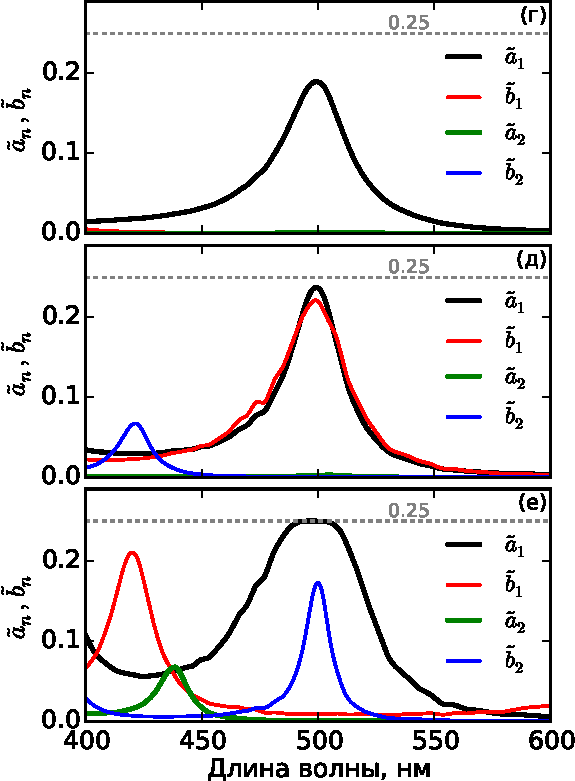
\includegraphics[height=1.35\linewidth]{2015-04-01-SiAgSi-ab-spectra4}}
  \end{minipage}
  \caption{ (а--в) Результат оптимизации эффективности поглощения
    $Si/Ag/Si$ наночастицей в зависимости от её внешнего радиуса, (а)
    эффективность поглощения, (б) коэффициенты поглощения в разложении
    Ми, где $\tilde{a}_1$ и $\tilde{a}_2$ относятся к электрическим, а
    $\tilde{b}_1$ и $\tilde{b}_2$ к магнитным диполю и квадруполю, (в)
    толщины составных слоёв наночастиц, (г--е) спектры коэффициентов
    поглощения в разложении Ми для дизайнов, соответствующих локальным
    максимумам на рисунке~\ref{img:q-abs}а.}
  \label{img:q-abs}  
\end{figure}


На рисунке~\ref{img:q-abs}(б) изображены значения коэффициентов Ми для
поглощения различными модами, горизонтальной пунктирной линией
отмечено значение теоретически достижимого предела, равное 1/4. В
случае небольшого размера оптимизированной частицы основной вклад в
поглощение даёт электрический диполь $\tilde{a}_1$.  Для дизайнов с
$R > 56.6$~нм оказалось, что поглощение одновременно на электрическом
и магнитном диполях позволяют достичь большего общего сечения
поглощения, чем в случае поглощения только электрическим
диполем. Такое качественное изменение соответствует разрывам линий на
рисунках~\ref{img:q-abs}(б--в) и реализует режим суперпоглощения.
Необходимо отметить, что для небольшого диапазона размеров частицы
$80.7<R<82.1$~нм оптимальное поглощение обеспечивает использование
электрического дипольного $\tilde{a}_1$ и магнитного квадрупольного
$\tilde{b}_2$ резонансов, что приводит ещё к двум разрывам линий на
рисунках для соответствующих значений внешнего радиуса~$R$.

На рисунке~\ref{img:q-abs}(в) представлены толщины составных слоёв
наночастицы, полученные в результате оптимизации эффективности
поглощения.  Неожиданно оказалось, что дизайны с преобладающим
дипольным механизмом поглощения (т.е. для размеров частицы менее
56.6~нм) могут быть двух видов.  Чтобы получить наилучшее поглощение
для $R<46$~нм, хватает использования всего двух слоёв, при оптимизации
толщина внутреннего слоя исходного трёхслойного дизайна обратилась в
ноль.  При $R=46$~нм поглощение диполем почти достигает своего
теоретического предела ($\tilde{a}_1>0.249$), чтобы удерживать его
вблизи этого значения для больших значений $R$, оптимизатор начинает
наращивать толщину внутреннего кремниевого слоя.  В свою очередь, это
приводит к появлению слабого поглощения  $\tilde{a}_2$,
что, впрочем, не позволяет достичь режима суперпоглощения для $n=2$.

Для расчёта спектров на рисунках~\ref{img:q-abs}(г--е) были
использованы экспериментальные дисперсионные зависимости для
показателей преломления из работы\cite{palik-1997}. Спектры для
коэффициентов поглощения в разложении Ми построены для случаев,
соответствующих локальным максимумам на рисунке~\ref{img:q-abs}(а),
дополнительно отмеченных стрелками.  Спектр для дизайна с внешним
радиусом $R=36$~нм на рисунке~\ref{img:q-abs}(г) подтверждает
дипольный характер поглощения с резонансом на выбранной для
оптимизации длины волны $\lambda=500$~нм.  Дизайны с
максимумами поглощения для $R=63$~нм и $R=81$~нм
(рисунки~\ref{img:q-abs}(д) и~\ref{img:q-abs}(е) соответственно)
обладают типичной для суперпоглощения структурой с вырождением
нескольких резонансов. На этих спектрах присутствуют дополнительные
резонансы, которые, впрочем, расположены в значительном отдалении от
выбранной для оптимизации длины волны, поэтому их вклад в общее
поглощение мал.

Для спектра на рисунке~\ref{img:q-abs}(е) несколько неожиданной
оказалась форма кривой для электрической дипольной моды, вершина
резонансного колокола выглядит практически плоской.  Были проведены
дополнительные расчёты, построены спектры для коэффициентов Ми для
каждого слоя. Для рассматриваемой оптимизированной структуры
оказалось, что максимумы электрических дипольных резонансов,
сопоставляемые каждому слою, находятся на разных длинах волн, их
суперпозиция и приводит к соответствующему уширению спектра
поглощения.

Особо надо отметить, что для получения максимальной эффективности
поглощения вовсе не требуется режима суперпоглощения.  Из
рисунка~\ref{img:q-abs}(а) следует, что максимальная эффективность
соответствует малым размерам частицы, где значение коэффициента Ми для
поглощения заметно меньше теоретического предела.  Среди всех
рассмотренных структур двухслойная частица $Ag/Si$ с внешним радиусом
36~нм обладает максимальной эффективностью поглощения.  Для неё
сечение поглощения более чем 5 раз превысило её геометрическое
сечение, хотя значение коэффициента $\tilde{a}_1$ меньше
фундаментального предела приблизительно на 20\%.  Этот результат
хорошо согласуется с выводами работы~\cite{Miller-2014}, где
эффективность поглощения, получаемя нормировкой на объём, оказалась
максимальной для частиц произвольной формы и небольшого размера с
преимущественным вкладом электрической дипольной моды.  Дополнительным
преимуществом двухслойных частиц может являться то, что они должны
быть проще и дешевле в производстве по сравнению с трёхслойными.  В то
же время для частиц большего размера ($R>60$~нм для рассмотренных
материалов) максимальная эффективность получается в режиме
суперпоглощения.  Это может оказаться существенно для случая, когда
изготовление многослойных частиц меньшего размера недоступно по
какой-либо технологической причине.

Основной вопрос, который возникает при обсуждении данных,
представленных на рисунке~\ref{img:q-abs}, касается достоверности
полученных результатов.  В первой главе диссертации уже была
верифицированна программа расчёта по теории Ми, это позволяет
утверждать, что полученные дизайны действительно обладают заявленными
значениями эффективности поглощения.  Во второй главе был подробно
рассмотрен используемый алгоритм оптимизации, на ряде примеров была
показана его эффективность.  Так как она зависит от вида
оптимизируемой функции, то вопрос можно переформулировать следующим
образом: насколько можно доверять результатам оптимизации в случае
поиска максимального значения функции эффективности поглощения
многослойной наночастией в зависимости от толщины составных слоёв?

Сами по себе численные методы оптимизации не могут гарантировать, что
будет найден глобальный экстремум целевой функции. Они успешно
могут применяться для частичного решения задачи о существовании,
являясь способом нахождения новых дизайнов с заранее заданными
свойствами или близкими к ним.  Недостатком выбраного подхода является
отсутствие доказательства единственности полученного решения.  Другими
словами, оптимизатор может терять какие-то решения (точнее, не
находить их), нет гарантий, что получаемый ответ является главным и
единственным экстремумом.

При решении физических и инженерных задач можно опираться на косвенные
признаки, сопутствующие оптимальному решению.  В случае, если такое
решение вступает в противоречие с какими-то заключениями других
методов, применяемых для рассмотрения изучаемой системы, то возникает
возможность получить новое знание либо о самой системе, либо об
особенностях её рассмотрения с помощью стохастического
оптимизатора. Возможна и другая ситуация, когда оптимальное решение,
полученное численными методами, обладает набором свойств, которые
могут быть предсказаны при аналитическом рассмотрении или при
качественном анализе системы. В этом случае приходится признать, что
предсказательная способность выбранного численного метода ни в чём не
уступает другим теоретическим методам и в рамках использованных
допущений получаемые результаты являются достоверными. Рассмотрим с
этой точки зрения представленные на рисунке~\ref{img:q-abs}
результаты.

Мощность поглощения света многослойными сферическими наночастицами
определяется как
\[
  P_{\mathrm {abs}}=\frac{1}{2}\int\sigma \left|E\right|^2dx\,dy\,dz,
\]
где локальная проводимость
$\sigma\propto \operatorname{\mathbb{I}m} (\epsilon)$ на выбранной
частоте падающего излучения слабо отличается у использованных
материалов ($Si$ и $Ag$).  Поэтому для получения максимального
поглощения для заданного внешнего размера в первую очередь выгодно
изменять дизайн наночастицы таким образом, чтобы возбуждение
происходило с максимально возможным усилением поля внутри частицы, то
есть резонансым образом.  Знание о таком способе увеличения поглощения
света наночастицей не передавалось в оптимизатор, который искал
наиболее подходящие дизайны для фиксированного значения длины волны и
внешнего радиуса сферы.  Другими словами, у оптимизатора не было
возможности ориентироваться на положение резонансов в спектре
поглощения. Фиксирование значение длины волны исключает возможность
прямого получения спектральных характеристик, фиксированный внешний
радиус наночастицы исключает возможность делать это косвенным образом,
применяя преобразование пространственного масштаба для уравнений
Максвелла. Однако если расчитать для полученных дизайнов спектр
зависимости коэффициентов поглощения от длины волны, то оказывается,
что условие резонансного возбуждение выполняется как раз для
оптимизируемой длины волны $\lambda=500$~нм,
см. рисунки~\ref{img:q-abs}~(г-е).  Это свидетельствует о том, что с
помощью численной оптимизации было получено правильное решение.

Как уже отмечалось, в своей работе~\cite{Tribelsky-2011}
М.И. Трибельский показал что существует верхний предел, ограничивающий
возможности поглощения для одного мультиполя; коэффициенты Ми для
поглощения $\tilde{a}_n$ и $\tilde{b}_n$ не могут превысить $1/4$,
близкие к этой величине значения соответствуют резонансному случаю,
без которого не получить высокой эффективности поглощения.  Метод
численной оптимизации не может провести подобный анализ.  Тем не
менее, когда частица оказывается достаточно большой, чтобы в ней можно
было возбудить электрическую дипольную моду, то для оптимизированных
дизайнов один или несколько коэффициентов Ми для поглощения имеет
значение в интервале от~0.2 до~0.25.  Это ещё  раз подтверждает
корректность выбранного подхода.

Для того, чтобы лучше понять влияние мультипольных резонансов на
эффективность поглощения был выполнен дополнительный прогон
оптимизации. В нём искались дизайны, обладающие максимальным значением
величины $\tilde{a}_1$, являющуюся коэффициентом Ми для поглощения
электрической дипольной модой. На рисунке~\ref{img:q-abs-a1}
приводится сравние двух прогонов оптимизации: (а--в) --- результаты,
соответствующие максимальному значению $Q_{abs}$ (полученого ранее),
(г--е) --- величине $\tilde{a}_1$.
\begin{figure}[t]
  \begin{minipage}[ht]{0.495\linewidth}
    \centering{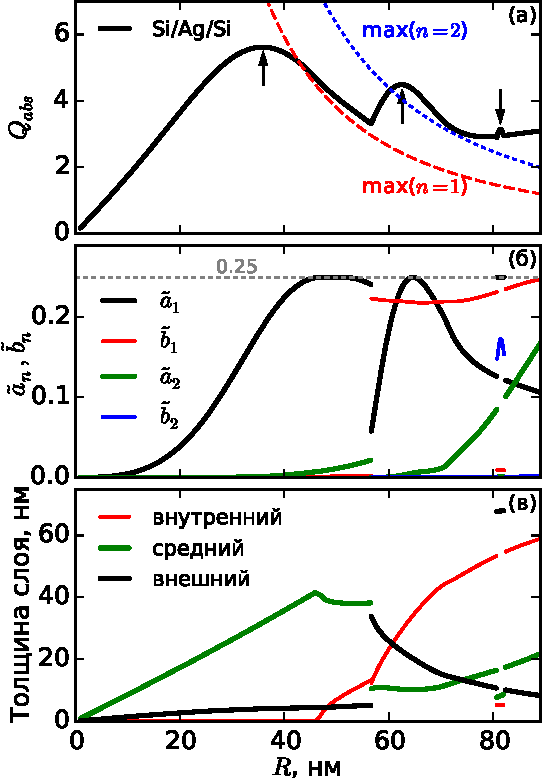
\includegraphics[width=0.95\linewidth]{2015-04-01-Qabs-SiAgSi-overview}}
  \end{minipage}
  \hfill
  \begin{minipage}[ht]{0.495\linewidth}
    \centering{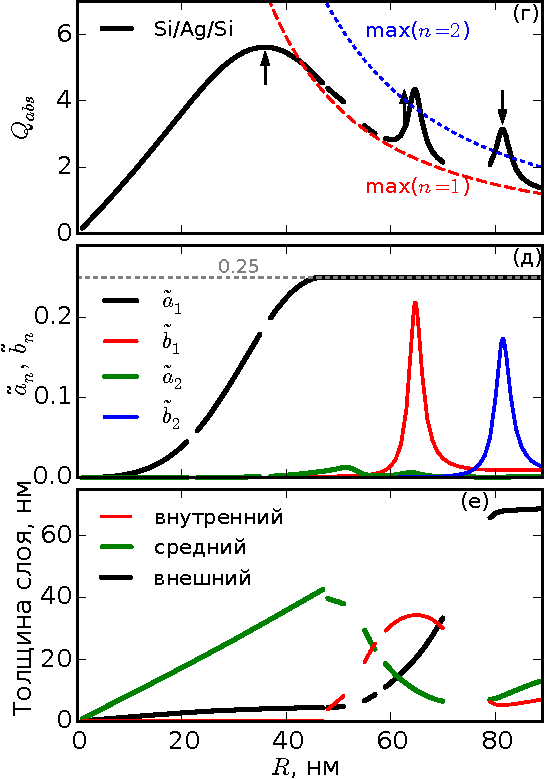
\includegraphics[width=0.95\linewidth]{overview-Qabs-a1-ru}}
  \end{minipage}
  \caption{ Результат оптимизации $Si/Ag/Si$ наночастицы в
    зависимости от её внешнего радиуса.  Копия
    рисунка~\ref{img:q-abs}(а--в), приводится для удобства сравнения
    оптимизации максимальной (а--в)~эффективности поглощения $Q_{abs}$
    и (г--е)~$\tilde{a}_1$, где (а,г)~эффективность
    поглощения, (б,д)~коэффициенты поглощения в разложении Ми, где
    $\tilde{a}_1$ и $\tilde{a}_2$ относятся к электрическим, а
    $\tilde{b}_1$ и $\tilde{b}_2$ к магнитным диполю и квадруполю,
    (в,е)~толщины составных слоёв наночастиц.}
  \label{img:q-abs-a1}
\end{figure}
Перед обсуждением полученных результатов необходимо сделать замечание
технического характрера.  С одной стороны, для корректного сравнения
этих двух случаев хотелось бы ограничиться минимальным изменением
параметров моделирования.  Сам по себе расчёт эффективности поглощения
по теории Ми уже требует предварительного расчёта всех коэффициентов
разложения, поэтому изменение оптимизируемой функции оказывается
тривиальным.  С другой стороны, расчёт такой зависимости являетсятся
достаточно трудоёмким с вычислительной точки зрения.  Так как этот
прогон оптимизации приводится только в целях верификации предлагаемого
подхода, то был выбран значительно более крупный шаг изменения
внешнего радиуса наночастцы.  Для всех зависимостей на
рисунке~\ref{img:q-abs-a1} был использован один и тот же критерий для
определения мест разрывов, реализованной в виде программы для
построения графиков.  Применение этого критерия в случае крупного шага
изменения по горизонтальной оси привело к серии ложных срабатываний,
часть точек оказалась отделена от сплошной кривой с обоих сторон
разрывом и не отображается на графке.  Наиболее наглядно такая
ситуация представлена на рисунке~\ref{img:q-abs-a1}(е), где для
значений внешнего радиуса $70<R<78$~нм отсутствует визуализация данных
о толщинах составных слоёв.  Так как подобные пробелы отсутствуют при
построении коэффициентов Ми для наиболее интересного диапазона внешних
радиусов наночастицы и не влияют на общий характер демонстрируемой
зависимости, то было принято решение не тратить время на доработку
алгоритма построения графиков.  Принимая во внимание эту техническую
особенность, можно сравнивать случаи $Q_{abs}$
(рисунок~\ref{img:q-abs-a1}(а--в)) и $\tilde{a}_1$
(рисунок~\ref{img:q-abs-a1}(г--е)) при оптимизации дизайна наночастицы
для получения максимального значения этих величин.

Для небольших значений внешнего радиуса наночастицы $R<45$~нм оба
случая оптимизации демонстрируют идентичные результаты. Это выглядит
логично, так как в отсутствие других мультиполей эффективность
поглощения полностью определяется электрической дипольной
модой. Другими словами для этого диапазона размеров максимальное
значение $Q_{abs}$ соответствует максимальному значению
$\tilde{a}_1$. Небольшое расхождение возникает после появления
третьего слоя и в основном проявляется в дизайне наночастицы.
Существенное различие становится заметно после того, как $\tilde{a}_1$
на рисунке~\ref{img:q-abs-a1}(б) начинает уменьшаться, что
приблизительно соответствует общему размеру $R=55$~нм. На
рисунке~\ref{img:q-abs-a1}(д) $\tilde{a}_1$ продолжает держаться
вблизи значения $1/4$, а вот сопутствующее значение $Q_{abs}$
оказывается несколько меньше. Такое поведение в полной мере отражает
различие в выбраной целевой функции двух прогонов
оптимизации. Промежутный результат можно сформулировать следующим
обрзом: даже в случае, когда поглощение происходит преимущенно на
дипольной моде, для получения максимальной эффективности поглощения
может быть выгодно иметь более сильную квадрупольную моду в ущерб
дипольной.

Интересно, что на рисунке~\ref{img:q-abs-a1}(д) при дальнейшем
увеличении внешнего размера оптимизированной наночастицы нарастают и
убывают вначале дипольная, а потом и квадрупольная магнитные моды. При
этом точка макимума дипольной магнитной моды соответствует
максимальному значению $Q_{abs}$, а дизайн наночастицы в этой точке
($R=65$~нм) совпадает у обоих прогонов оптимизации
рисунка~\ref{img:q-abs-a1}.  Аналогичная ситуация и вблизи максимума
квадрупольной магнитной моды, где совпадение наблюдается для диапазона
$80.7<R<82.1$~нм.  Всё вместе это ещё раз свидетельствует о верности
выбранного подхода: результаты, полученные при оптимизации с
использованием разных целевых функций, оказались согласованны между
собой.





\begin{figure}[t]
  \centering{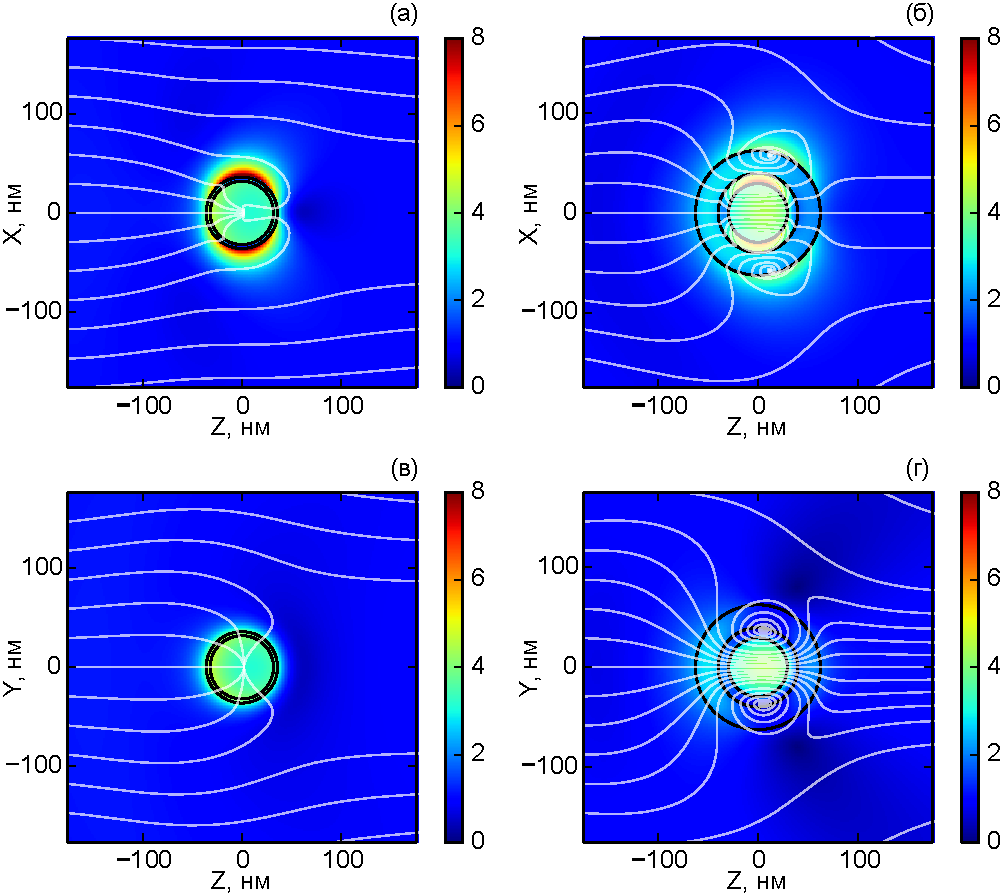
\includegraphics[width=0.95\linewidth]{SiAgSi-flow-YZ-Eabs-ru}}
  \caption{ (а--в) Результат оптимизации эффективности поглощения
    $Si/Ag/Si$ наночастицей в зависимости от её внешнего радиуса, (а)
    эффективность поглощения, (б) коэффициенты поглощения в разложении
    Ми, где $\tilde{a}_1$ и $\tilde{a}_2$ относятся к электрическим, а
    $\tilde{b}_1$ и $\tilde{b}_2$ к магнитным диполю и квадруполю, (в)
    толщины составных слоёв наночастиц, (г--е) спектры коэффициентов
    поглощения в разложении Ми для дизайнов, соответствующих локальным
    максимумам на рисунке~\ref{img:q-abs}а.}
  \label{img:absorb-field}  

\end{figure}


The stochastic algorithm utilized in our approach is very generic and
the optimization can be repeated for any desired wavelength or
wavelength range.  As a result, one can design spectrally-selective
absorbers or broadband absorbers with almost arbitrary prescribed
properties. We note, that using this algorithm, one can optimize not
only absorbtion efficiency, but also other parameters that may be
desired for some applications. As an example we reproduce some of the
results from the work of Estakhri and Al\`u,\cite{Alu-2014} where
authors aim to design absorbers with small scattering cross-section,
and we provide a number of new optimized designs. The efficiency in
the Ref.\cite{Alu-2014} is defined as the ACS normalized to
scattering cross-section. Initially, we set the total value of the
absorbed power with cross-section of $\alpha_{\mathrm
  abs}=\frac{3\lambda^2}{8\pi}$ and keep the outer radius of the
particle fixed. In this case the optimization gives a result similar
to the structure with contributing harmonics TM${_1}$ and TE$_1$ from
Ref.\cite{Alu-2014}  For $\epsilon_1 = 1.29+i0.01$, $\epsilon_2 =
-10.37+ i0.35$, and $\epsilon_3=8.4+i2.33$ as material parameters we
obtained radii $\{a_{c1},a_{c2},a_3\}=\{0.142,0.166,0.194\}\lambda$
and scattering-normalized absorption efficiency $\eta_{\mathrm
  abs}^{(\alpha)} =7.65$ which corresponds to $\eta_{\mathrm
  abs}^{(\alpha)} =7.1$ from the original work.\cite{Alu-2014}
However, if we set the optimizer to keep high level of absoption
efficiency $Q_{\mathrm abs} \approx 5$ the particle becomes much smaller
and the size of the outer layer vanishes
$\{a_{c1},a_{c2}\}=\{0.00635,0.00747\}\lambda$ resulting in $\eta_{\mathrm
  abs}^{(Q)} =544$.  It means that this small particle still absorbs
five times its phisical size with a very large scattering-normalized
absorption efficiency.


\section{Выводы}



\clearpage